\subsection{Zerfallskan�le von $\mu$, $\pi$ und $K$}
Im Folgenden sind die Zerfallskan�le von $\mu$, $\pi$ und $K$ bzw. in diesem Fall die wahrscheinlichsten Zerfallsprodukte dargestellt.(vgl. \cite{perkins} Seite 406 ff.)
\begin{table}[H]
\caption{Zerfallskan�le von $\mu$, $\pi$ und $K$}
\label{tab:zerfallskan�le}
\centering
\begin{tabular}{|c|c|c|c|c|c|}
\hline Particle & $J^P$ & $\frac{m_0}{\text{MeV}}$ & $\frac{\tau}{\text{s}}$ & Decay & Fraction \\ 
\hline $\mu^{\pm}$ & $\frac{1}{2}$ & $105.6595(\pm 2)$ & $2.1971(\pm 1)\times10^{-6}$ & $e \nu \bar{\nu}$ & $\SI{100}{\percent}$ \\
\hline
\hline $\pi^{\pm}$ & $0^-$ & $139.567(\pm 1)$ & $2.603(\pm 2)\times 10^{-8}$ & $\mu \nu$ & $\simeq \SI{100}{\percent}$ \\
\hline
\hline $\pi^{0}$ & $0^-$ & $134.963(\pm 4)$ & $0.83(\pm 6)\times 10^{-16}$ & $\gamma \gamma$ & $\SI{98.8}{\percent}$ \\
\hline  &  &  &  & $\gamma e^+ e^-$& \SI{1.17}{\percent} \\
\hline
\hline $K^{\pm}$ & $0^-$ & $493.67(\pm 2)$ & $1.237(\pm 3) \times 10^{-8}$ & $\mu^{\pm} \nu$ & \SI{63.5}{\percent} \\
\hline  &  &  &  & $\pi^{\pm} \pi^0$& \SI{21.2}{\percent} \\
\hline  &  &  &  & $\pi^{\pm} \pi^+ \pi^-$& \SI{5.6}{\percent} \\
\hline  &  &  &  & $\pi^{\pm} \pi^{0} \pi^{0}$& \SI{1.7}{\percent} \\
\hline  &  &  &  & $\mu^{\pm} \pi^{0} \nu$& \SI{3.2}{\percent} \\
\hline  &  &  &  & $e^{\pm} \pi^0 \nu$ & \SI{4.8}{\percent} \\
\hline
\hline $K^{0} , \bar{K^{0}}$ & $0^-$ & $497.7(\pm 1)$ & $K_S: 0.892(\pm 2) \times 10^{-10}$ $K_L: 5.18(\pm 4) \times 10^{-8}$ & & \\
\hline
\hline $K_S$ &&&& $\pi^+ \pi^-$ & \SI{68.6}{\percent} \\
\hline &&&& $\pi^0 \pi^0$ & \SI{31.3}{\percent} \\
\hline
\hline $K_L$ &&&& $\pi^0 \pi^0 \pi^0$ & \SI{21.5}{\percent} \\
\hline &&&& $\pi^+ \pi^- \pi^0$ & \SI{12.6}{\percent} \\
\hline &&&& $\pi \mu \nu$ & \SI{26.8}{\percent} \\
\hline &&&& $\pi e \nu$ & \SI{38.8}{\percent} \\
\hline
\end{tabular}
\end{table}
\noindent
$\tau$ entspricht dabei der mittleren Lebensdauer. Das Feynman-Diagramm f�r den Zerfall eines Myuons ist in Abb. \ref{fig:myon_zerfall} dargestellt. (vgl. \cite{wiki_myon})
\begin{figure}[H]
\centering
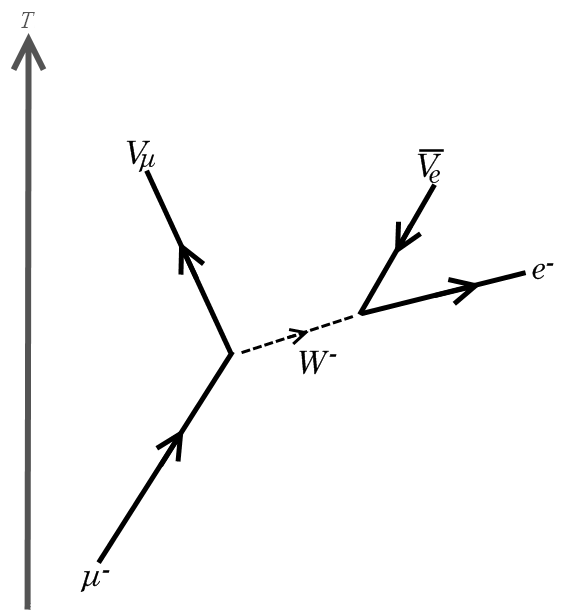
\includegraphics[scale = 1]{Muon_Decay.png}
\caption{Myon Zerfallskanal}
\label{fig:myon_zerfall}
\end{figure}
Pionen sind aus einem u-d Paar aufgebaut und Kaonen aus einem u-s oder d-s Paar. Die Teilchen mit unterschiedlichen Indizes unterscheiden sich in der Kombination von Quark und Antiquark, auf die hier nicht genauer eingegangen werden soll. Myonen entstehen in etwa 10 bis 15 km H�he aus Zerf�llen von Pionen und Kaonen. Kosmische Strahlung besteht zu einem gro�en Teil aus Spallationsprozessen von Protonen (z.B. aus Sonnenwinden) in der oberen Atmosph�re. Die Targets werden aufgrund der hohen Energie von den Protonen zerschlagen und es entsteht ein sogenannter Teilchenschauer. In Abb. \ref{fig:teilchenschauer} ist ein solcher Schauer dargestellt.\\(vgl. \cite{auger_teilchenschauer})
\begin{figure}[H]
\centering
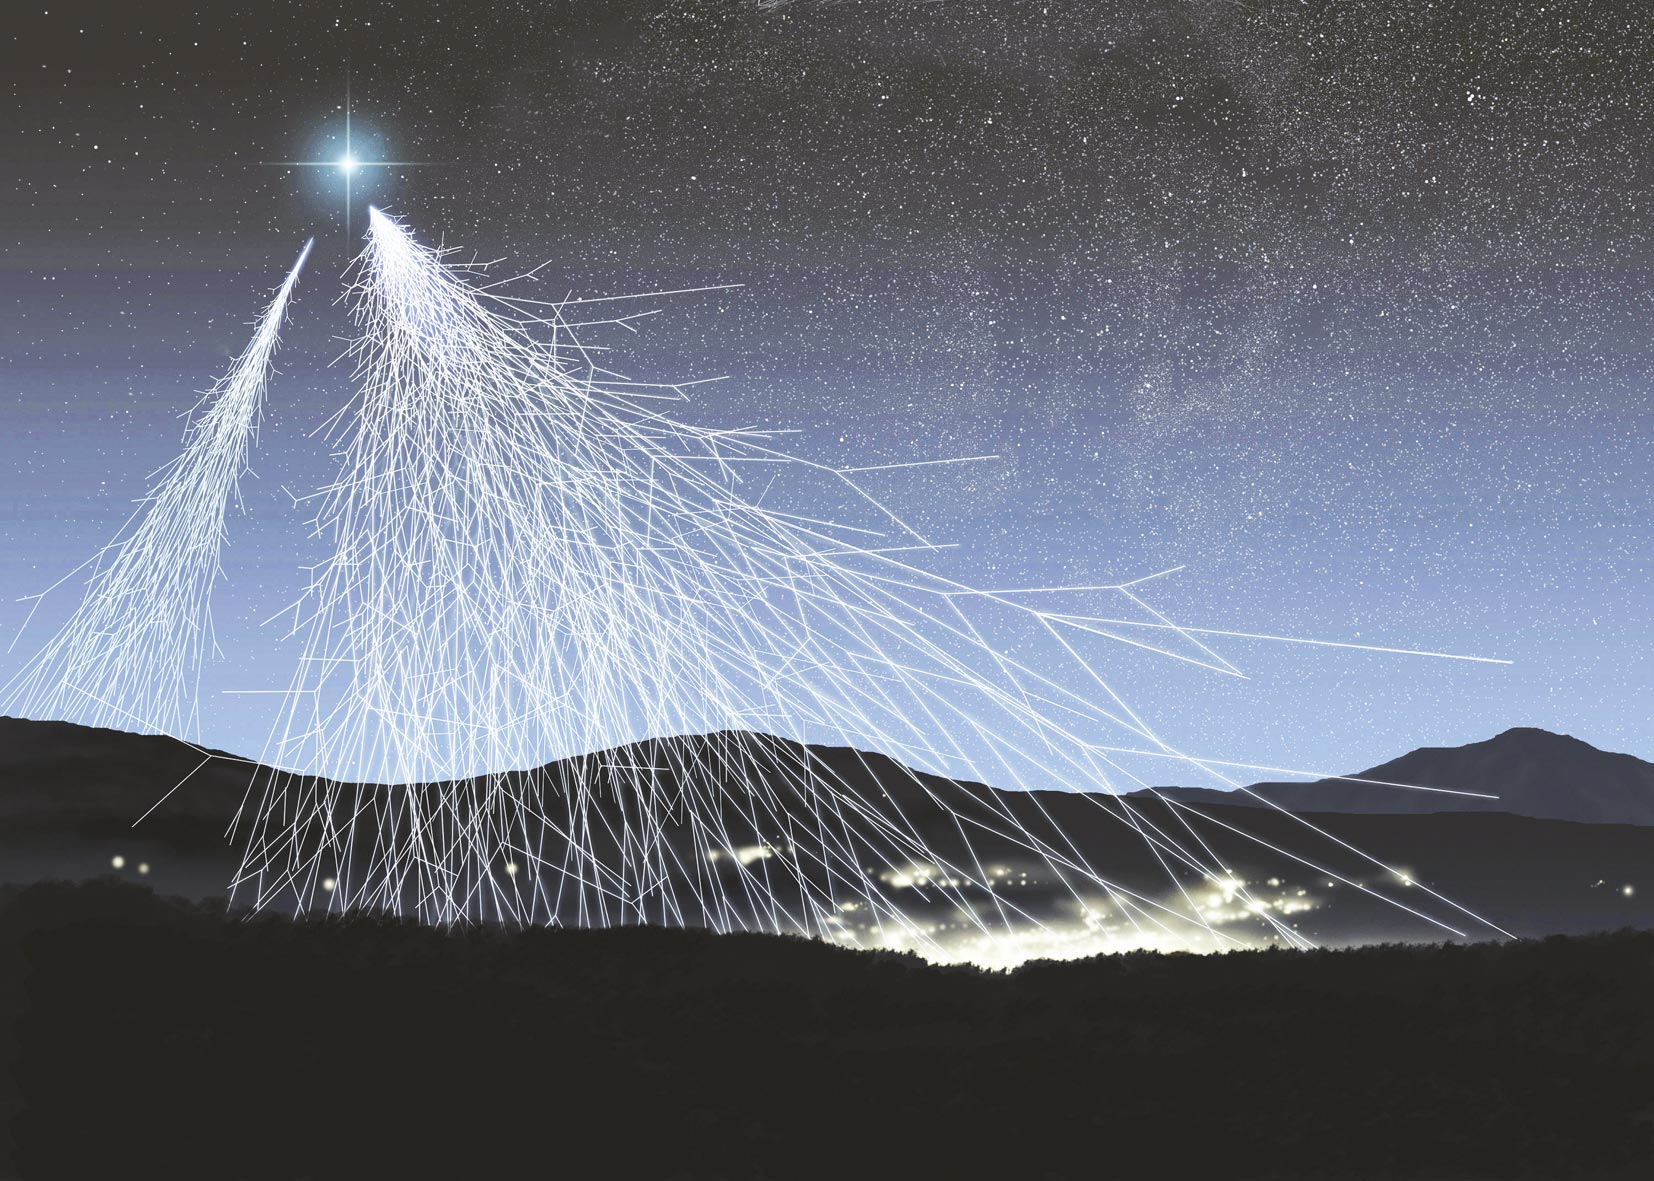
\includegraphics[scale = 0.3]{cosmicray_}
\caption{Teilchenschauer}
\label{fig:teilchenschauer}
\end{figure}